% The 2-adic integers as a binary tree of balls. Generated by a short script.
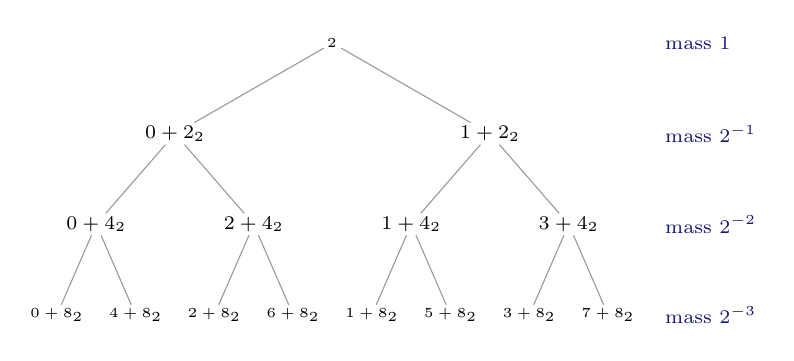
\begin{tikzpicture}[xscale=1.0,yscale=1.15]
\node[font=\scriptsize,fill=white,inner sep=1pt] (n00) at (4.000,0) {$\Z_2$};
\node[font=\scriptsize,right,MidnightBlue] at (8.1,0) {mass $1$};
\node[font=\scriptsize,fill=white,inner sep=1pt] (n10) at (2.000,-1) {$0+2\Z_2$};
\draw[black!40] (n00) -- (n10);
\node[font=\scriptsize,fill=white,inner sep=1pt] (n11) at (6.000,-1) {$1+2\Z_2$};
\draw[black!40] (n00) -- (n11);
\node[font=\scriptsize,right,MidnightBlue] at (8.1,-1) {mass $2^{-1}$};
\node[font=\scriptsize,fill=white,inner sep=1pt] (n20) at (1.000,-2) {$0+4\Z_2$};
\draw[black!40] (n10) -- (n20);
\node[font=\scriptsize,fill=white,inner sep=1pt] (n21) at (3.000,-2) {$2+4\Z_2$};
\draw[black!40] (n10) -- (n21);
\node[font=\scriptsize,fill=white,inner sep=1pt] (n22) at (5.000,-2) {$1+4\Z_2$};
\draw[black!40] (n11) -- (n22);
\node[font=\scriptsize,fill=white,inner sep=1pt] (n23) at (7.000,-2) {$3+4\Z_2$};
\draw[black!40] (n11) -- (n23);
\node[font=\scriptsize,right,MidnightBlue] at (8.1,-2) {mass $2^{-2}$};
\node[font=\tiny,fill=white,inner sep=1pt] (n30) at (0.500,-3) {$0+8\Z_2$};
\draw[black!40] (n20) -- (n30);
\node[font=\tiny,fill=white,inner sep=1pt] (n31) at (1.500,-3) {$4+8\Z_2$};
\draw[black!40] (n20) -- (n31);
\node[font=\tiny,fill=white,inner sep=1pt] (n32) at (2.500,-3) {$2+8\Z_2$};
\draw[black!40] (n21) -- (n32);
\node[font=\tiny,fill=white,inner sep=1pt] (n33) at (3.500,-3) {$6+8\Z_2$};
\draw[black!40] (n21) -- (n33);
\node[font=\tiny,fill=white,inner sep=1pt] (n34) at (4.500,-3) {$1+8\Z_2$};
\draw[black!40] (n22) -- (n34);
\node[font=\tiny,fill=white,inner sep=1pt] (n35) at (5.500,-3) {$5+8\Z_2$};
\draw[black!40] (n22) -- (n35);
\node[font=\tiny,fill=white,inner sep=1pt] (n36) at (6.500,-3) {$3+8\Z_2$};
\draw[black!40] (n23) -- (n36);
\node[font=\tiny,fill=white,inner sep=1pt] (n37) at (7.500,-3) {$7+8\Z_2$};
\draw[black!40] (n23) -- (n37);
\node[font=\scriptsize,right,MidnightBlue] at (8.1,-3) {mass $2^{-3}$};
\end{tikzpicture}
